% Convergence of the hundredth eigenvalue against the degrees of freedom,
% triangular domain: the eigenvalue itself on the left, the relative error on
% the right.
%
% Requires in the preamble:
%   \usepackage{graphicx}
%   \usepackage{subfig}
%   \usepackage{epstopdf}   % the figures are EPS; needed under pdflatex,
%                           % which then wants -shell-escape. Not needed for
%                           % latex/dvips, which reads EPS directly.
%
% The figures live next to this file, in
% results_paper/eigenvalues_convergence/. If you \input this snippet
% from elsewhere, point graphicx at that folder, e.g.
%   \graphicspath{{results_paper/eigenvalues_convergence/}}
% and drop the leading path from the \includegraphics arguments below.

\begin{figure}[htbp]
  \centering
  \subfloat[Eigenvalue $\lambda_{100}$.\label{fig:convergence_isosceles_triangle_lambda100_value}]{%
    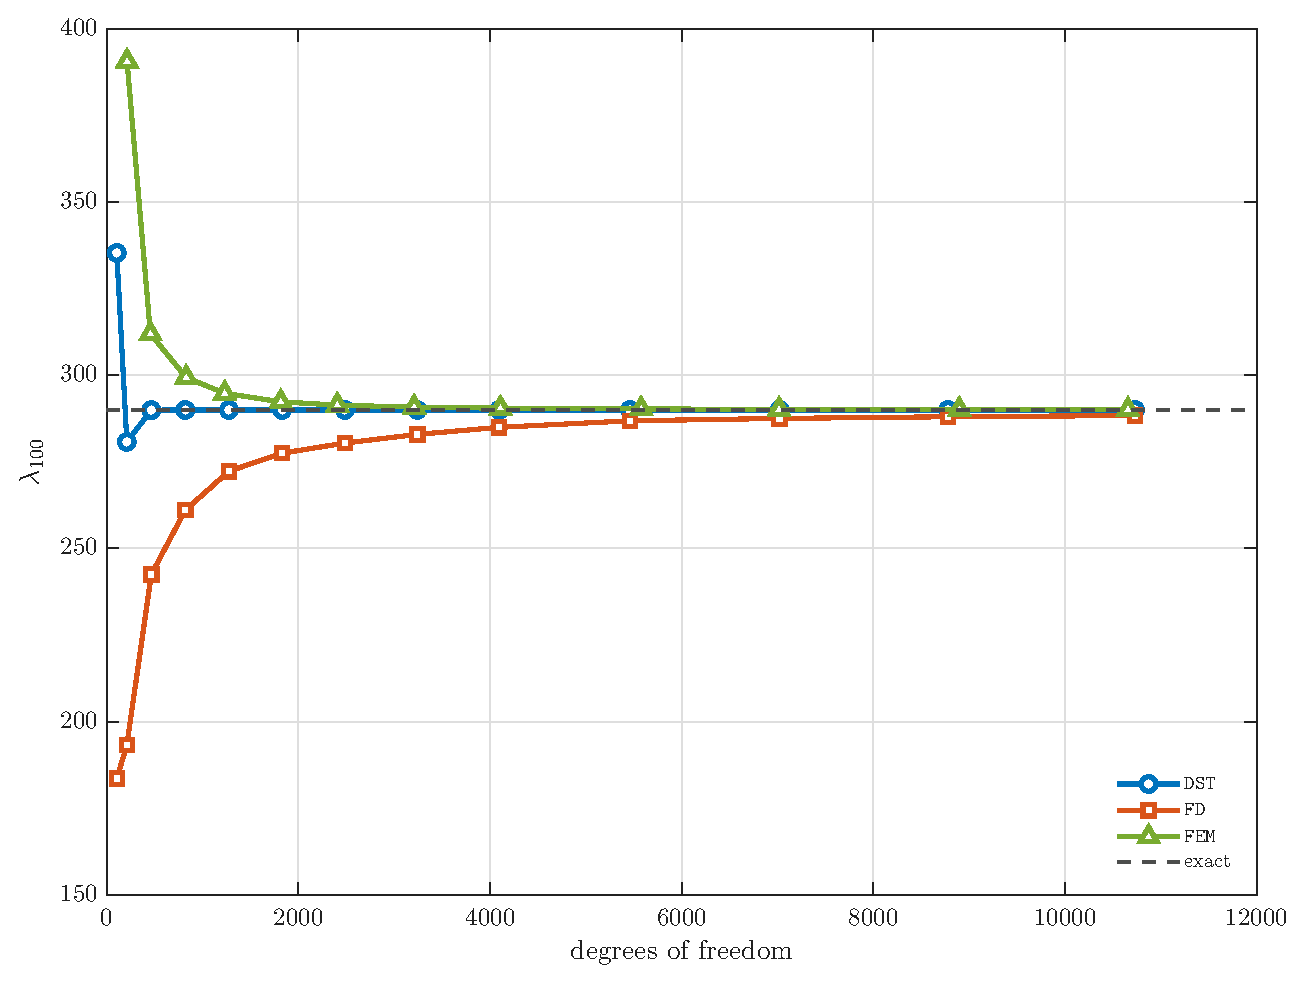
\includegraphics[width=0.45\textwidth]{isosceles_triangle_convergence_lambda100}}
  \qquad
  \subfloat[Relative error $\frac{|\lambda_{100} - \lambda_{100}^{\text{exact}}|}{\lambda_{100}^{\text{exact}}}$.\label{fig:convergence_isosceles_triangle_lambda100_error}]{%
    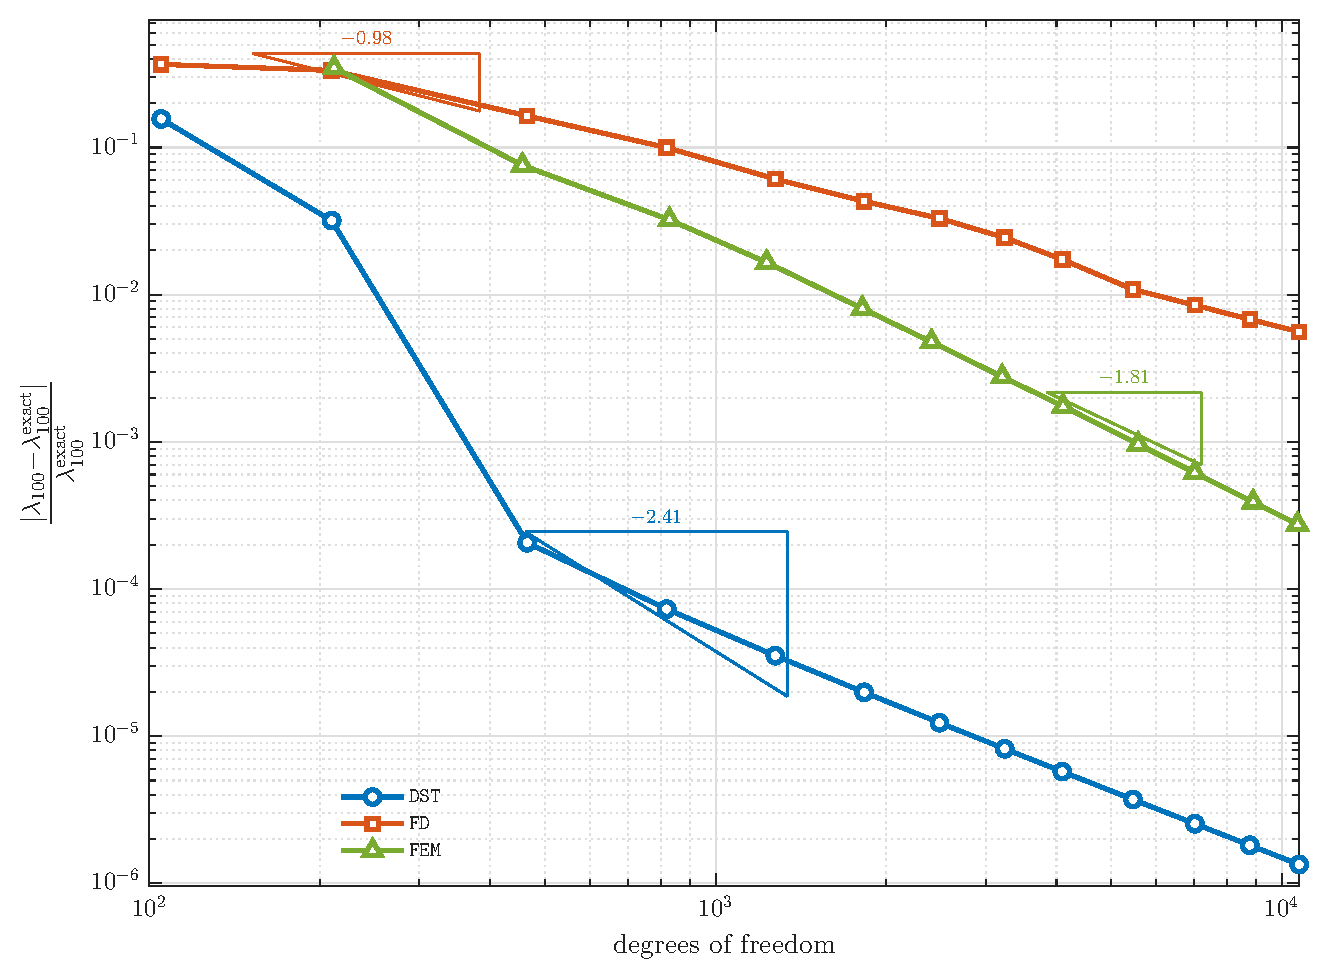
\includegraphics[width=0.45\textwidth]{isosceles_triangle_convergence_lambda100_error}}
  \caption{The hundredth eigenvalue $\lambda_{100}$ of Laplace operator, zero Dirichlet boundary conditions, triangular domain \texttt{isosceles\_triangle}, the right isosceles triangle with legs of length $\pi$. Eigenvalue $\lambda_{100}$ computed by each discretisation \texttt{DST}, \texttt{FD} and \texttt{FEM} with varying degrees of freedom; compared with the exact eigenvalue $\lambda_{100}^{\text{exact}}$, the hundredth value of $m^2 + n^2$, $m > n \geq 1$, in ascending order. Resolutions carrying fewer than 100 degrees of freedom cannot supply the eigenvalue and are left out.}
  \label{fig:convergence_isosceles_triangle_lambda100}
\end{figure}
